%Outline
%\begin{itemize}
%	\item Graph definition
%	\item Agent definition
%	\item Solution
%	\begin{itemize}
%		\item Explanation: a pathlike object
%		\item Definition: (c$_1$ ... c$_n$)
%		\item Constraints: where c1 = start, cn = goal, legal transitions
%	\end{itemize}
%	\item Remaining formalization
%\end{itemize}

\section{Problem definition}\label{sec:problem_definition}
Consider the set of traversal directions $D = \{north, south, east, west\}$  and a list of $m$ cells $C = (c_1, ..., c_m)$. 
The Flatland environment is defined as a tuple $(G,A)$ in which $G$ is a directed graph $G = (V,E)$, such that $V = C \times D$ and $E \subseteq V \times V$, and $A$ is a list of $n$ agents $A = (a_1, ..., a_n)$.
Each agent $a_i \in A$ is associated with a start vertex $s_i \in V$ and a set of target vertices $T \subset V$.
Time is considered discrete; between two consecutive timesteps, an agent can either move to another vertex (move action) or stay at its current vertex (wait action).  
Additionally, each agent $a_i$ is assigned a departure time $\delta_i$ and an arrival time $\alpha_i$; it is between only these time steps that the agent is permitted to execute move actions.
A valid solution path $\pi_i$ of agent $a_i$ is a finite sequence $(v_j)_{j=1}^k$ of vertices $v_j \in V$ for $0 \leq j \leq k$ such that $(v_j,v_{j+1}) \in E$ for all $0 \leq j \leq k$, as well as that $v_1 = s_i$ and $v_k \in T$.

\subsection{Example}\label{sec:example}
%The Flatland environment is represented as a grid to resemble a true railway network.
%This paper, however, represents the environment as a graph because of several advantages that will be discussed later in detail.
%Therefore, it is important to understand how the transformation from a grid to a graph occurs.
%A single cell contains a track which 

\begin{figure}[h!]
%\centering
        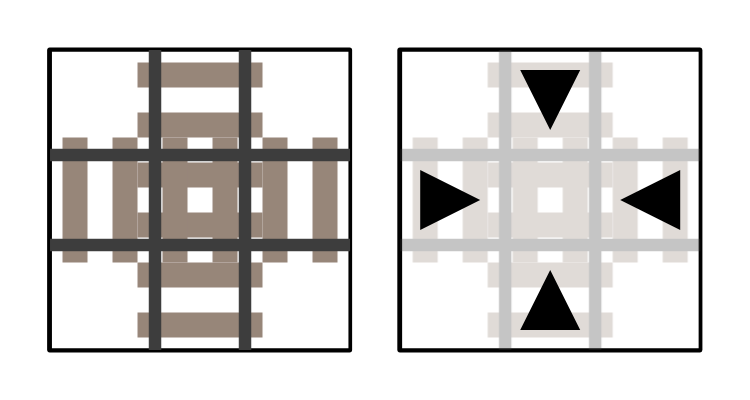
\includegraphics[width=.35\linewidth]{img/cross_both.png}
    \caption{ Each cell can contain up to four vertices, which correspond to the four traversal directions. Visually, the vertices in the figure represent the traversal direction the train is facing when it enters the cell. }
    \label{fig:verticalcell}
\end{figure}

\begin{figure}[h!]
%\centering
        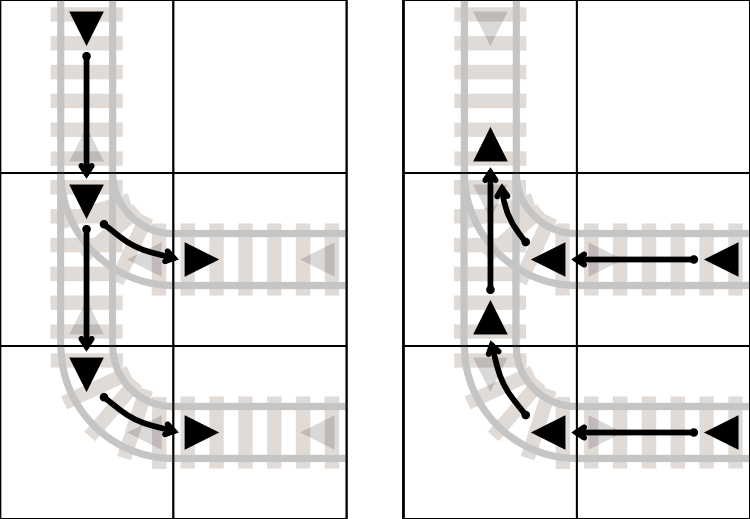
\includegraphics[width=.5\linewidth]{img/env_both.png}
    \caption{ For simplicity, the figure is split into two images: the first with edges in one direction, and the second with edges in the other direction.  Each vertex connects to at least one vertex belonging to another cell. } % In cases where a switch diverges, the vertex that represents a train facing the switch will have two outgoing edges. In cases where a switch converges, a vertex will have two incoming edges.
    \label{fig:verticalcell}
\end{figure}
